\documentclass[12pt,twocolumn,twoside]{book}

\usepackage{ebgaramond}
\usepackage[T1]{fontenc}
\usepackage{titlesec, xcolor}
\usepackage[spanish]{babel}
\usepackage{lettrine}
\usepackage{graphicx}
\usepackage{afterpage}
\usepackage[protestant]{bibleref-spanish}
\usepackage{indextools}

%for chapter headings
\definecolor{gray75}{gray}{0.75}
\newcommand{\hsp}{\hspace{20pt}} 
\titleformat{\chapter}[hang]{\Huge\bfseries}{\thechapter\hsp\textcolor{gray75}{|}\hsp}{0pt}{\Huge\bfseries}

%eliminate widows and orphans
%\widowpenalty=10000
%\clubpenalty=10000

% bible references
\newcommand{\cbibleref}[3]{\textbf{\ibibleverse[textit]{#1}(#2)}\ {#3}}
\newcommand{\cbiblechvs}[3]{\textbf{\ibiblechvs[textit]{#1}{#2}}\ {#3}}
\newcommand{\cbiblevs}[3]{\textbf{\ibiblechvs[textit]{#1}{#2}}\ {#3}}

\newcommand{\cbiblefoot}[3]{\footnote{\cbibleref{#1}{#2}{#3}}}
\newcommand{\cbiblefootduo}[6]{\footnote{\cbibleref{#1}{#2}{#3}\ldots \cbibleref{#4}{#5}{#6}}}
\newcommand{\cbiblefoottrio}[9]{\footnote{\cbibleref{#1}{#2}{#3}\ldots \cbibleref{#4}{#5}{#6}\ldots \cbibleref{#7}{#8}{#9}}}

\newcommand{\cbiblefootduosb}[5]{\footnote{\cbibleref{#1}{#2}{#3}\ldots \cbiblechvs{#1}{#4}{#5}}} %footnote with two texts from same book
\newcommand{\cbiblefoottriosb}[7]{\footnote{\cbibleref{#1}{#2}{#3}\ldots \cbiblechvs{#1}{#4}{#5}\ldots \cbiblechvs{#1}{#6}{#7}}}
\newcommand{\cbiblefootcuartosb}[9]{\footnote{\cbibleref{#1}{#2}{#3}\ldots \cbiblechvs{#1}{#4}{#5}\ldots \cbiblechvs{#1}{#6}{#7}\ldots \cbiblechvs{#1}{#8}{#9}}}

%title	
\providecommand{\HUGE}{\Huge}
\newlength{\drop}
\newcommand*{\titleGM}{\begingroup% Gentle Madness
\drop = 0.1\textheight
\vspace{\baselineskip}
\vfill
	\hbox{%
	\hspace*{0.2\textwidth}%
	\rule{1pt}{\textheight}
	\hspace*{0.05\textwidth}%
	\parbox[b]{0.75\textwidth}{
	\vbox{%
		\vspace{\drop}
		{\noindent\HUGE\bfseries\textcolor{red}{La Revelación}\\[0.5\baselineskip]\textcolor{red}{de Jesucristo}}\\\\
		{\Large\itshape Leyendola en la Luz del Antiguo Testamento}\\[4\baselineskip]		
		{\noindent Arreglado por Caleb George}\par
		\vspace{0.4\textheight}
		{\textbf{Kephali Press}}\\[\baselineskip]
		}% end of vbox
		}% end of parbox
	}% end of hbox
\vfill
\endgroup}

%dedication
\providecommand{\HUGE}{\Huge}
\newcommand*{\dedication}{\begingroup% Gentle Madness
\drop = 0.1\textheight
\vspace{\baselineskip}
\vfill
	\hbox{%
	\hspace*{0.2\textwidth}%
	\rule{0pt}{\textheight}
	\hspace*{0.05\textwidth}%
	\parbox[b]{0.75\textwidth}{
	\vbox{%
		\vspace{2\drop}	
		\begin{flushright}	
		{\Large\itshape Para Mi Amada Mabeliz}\\[1\baselineskip]		
		{\noindent\itshape Para ayudarte en tus esfuerzos por entender las Sagradas Escrituras}\par
		\end{flushright}
		\vspace{0.4\textheight}
		}% end of vbox
		}% end of parbox
	}% end of hbox
\vfill
\endgroup}

%verse numbers
\newcommand{\vnum}[1]{\textcolor{red}{\normalsize{#1}}}

%empty page
\newcommand{\blankpage}{\newpage
\thispagestyle{plain} % empty
\mbox{}}

% lettrine
\newcount\zzc
\makeatletter
\def\zz{%
\ifnum\prevgraf<\c@L@lines
\zzc\z@
\loop
\ifnum\zzc<\prevgraf
\advance\zzc\@ne
\afterassignment\zzda\count@\L@parshape\relax
\repeat
\parshape\L@parshape
\fi}
\def\zzda{\afterassignment\zzdb\dimen@}
\def\zzdb{\afterassignment\zzdef\dimen@}
\def\zzdef#1\relax{\edef\L@parshape{\the\numexpr\count@-1\relax\space #1}}
\makeatother
\usepackage{lettrine}

%index
\biblerefmap{Genesis}{01}
\biblerefmap{Exodus}{02}
\biblerefmap{Leviticus}{03}
\biblerefmap{Numbers}{04}
\biblerefmap{Deuteronomy}{05}
\biblerefmap{Joshua}{06}
\biblerefmap{Judges}{07}
\biblerefmap{Ruth}{08}
\biblerefmap{ISamuel}{09}
\biblerefmap{IISamuel}{10}
\biblerefmap{IKings}{11}
\biblerefmap{IIKings}{12}
\biblerefmap{IChronicles}{13}
\biblerefmap{IIChronicles}{14}
\biblerefmap{Ezra}{15}
\biblerefmap{Nehemiah}{16}
\biblerefmap{Esther}{17}
\biblerefmap{Job}{18}
\biblerefmap{Psalms}{19}
\biblerefmap{Proverbs}{20}
\biblerefmap{Ecclesiastes}{21}
\biblerefmap{Song of Solomon}{22}
\biblerefmap{Isaiah}{23}
\biblerefmap{Jeremiah}{24}
\biblerefmap{Lamentations}{25}
\biblerefmap{Ezekiel}{26}
\biblerefmap{Daniel}{27}
\biblerefmap{Hosea}{28}
\biblerefmap{Joel}{29}
\biblerefmap{Am}{30}
\biblerefmap{Obadiah}{31}
\biblerefmap{Jonah}{32}
\biblerefmap{Micah}{33}
\biblerefmap{Nahum}{34}
\biblerefmap{Habakkuk}{35}
\biblerefmap{Zephaniah}{36}
\biblerefmap{Haggai}{37}
\biblerefmap{Zachariah}{38}
\biblerefmap{Malachi}{39}

\makeindex[title=\'Indice de Escrituras,name=scr]
\makeindex[title=\'Indice General]
\renewcommand{\biblerefindex}{\index[scr]}

\begin{document}
\pagestyle{empty}
\frontmatter
\titleGM
\clearpage
\blankpage
\clearpage
\clearpage
\dedication
\clearpage
\tableofcontents
\clearpage
\listoffigures
\clearpage
\begin{figure*}[p!]
	\centering
       \includegraphics[scale=0.8]{Durer/durerRev1.png}    
    	\caption{La Visión de San Juan de los Siete Candelabros. Albrecht Dürer, 1498.}
    	\label{fig:candlesticks}
\end{figure*}
\pagestyle{headings}
\mainmatter

\chapter{Visión del Hijo del Hombre}
\lettrine[lines=4]{\textcolor{red}{L}}{ a Revelación}%
	\cbiblefootduo{Daniel}{2:28}{Pero hay un Dios en el cielo que revela los misterios, y Él ha dado a conocer al rey Nabucodonosor lo que sucederá al fin de los días}%
			{Amos}{3:7}{Ciertamente el Señor Dios no hace nada sin revelar Su secreto a Sus siervos los profetas} %
de Jesucristo, que Dios le dio, para mostrar a Sus siervos las cosas que deben suceder pronto. Él la dio a conocer enviándola por medio de Su ángel a Su siervo Juan, %
\vnum{2} quien dio testimonio de la palabra de Dios y del testimonio de Jesucristo, y de todo lo que vio. %
\vnum{3} Bienaventurado el que lee y los que oyen las palabras de la profecía y guardan las cosas que están escritas en ella, porque el tiempo está cerca.
\subsubsection*{Saludo a las siete iglesias}
\vnum{4} Juan, a las siete iglesias que están en Asia: Gracia y paz a ustedes, de parte de Aquel que es%
	\cbiblefoot{Exodus}{3:14}{Y dijo Dios a Moisés: «YO SOY EL QUE SOY»} %
y que era y que ha de venir, y de parte de los siete Espíritus%
	\cbiblefoot{Isaiah}{11:2}{Y reposará sobre Él el Espíritu del Señor, Espíritu de sabiduría y de inteligencia, Espíritu de consejo y de poder, Espíritu de conocimiento y de temor del Señor}%
que están delante de Su trono, %
\vnum{5} y de parte de Jesucristo, el testigo fiel, el primogénito%
	\cbiblefoot{Psalms}{87:28}{Yo también lo haré Mi primogénito, El más excelso de los reyes de la tierra} %
de los muertos y el soberano de los reyes de la tierra.%
	\cbiblefoot{Daniel}{7:14}{Y le fue dado dominio, gloria y reino, para que todos los pueblos, naciones y lenguas le sirvieran. Su dominio es un dominio eterno que nunca pasará, y Su reino uno que no será destruido}%
Al que nos ama%
	\cbiblefootduosb{Deuteronomy}{7:8}{mas porque el Señor los amó y guardó el juramento que hizo a sus padres, el Señor los sacó con mano fuerte y los redimió de casa de servidumbre, de la mano de Faraón, rey de Egipto}%
				{23:5}{el Señor tu Dios te cambió la maldición en bendición, porque el Señor tu Dios te ama} %
y nos libertó de nuestros pecados con Su sangre, %
\vnum{6} e hizo de nosotros un reino, sacerdotes%
	\cbiblefootduo{Exodus}{19:6}{Ustedes serán para Mí un reino de sacerdotes y una nación santa}%
				{Isaiah}{61:6}{Y ustedes serán llamados sacerdotes del Señor; ministros de nuestro Dios se les llamará. comerán las riquezas de las naciones, y en su gloria se jactarán} %
para Dios, Su Padre, a Él sea la gloria y el dominio por los siglos de los siglos. Amén. %
	\cbiblefoot{Psalms}{72:18-19}{Bendito sea el Señor Dios\ldots Bendito sea Su glorioso nombre para siempre, sea llena de Su gloria toda la tierra. Amén y amén.}
\parbox{.5\textwidth}{\begin{verse}\vnum{7} Él viene con las nubes,%
	\footnote{\cbibleref{Psalms}{18:10-12}{También inclinó los cielos, y descendió con densas tinieblas debajo de Sus pies. Cabalgó sobre un querubín, y voló; y rápido voló sobre las alas del viento. De las tinieblas hizo Su escondedero, Su pabellón a Su alrededor; tinieblas de las aguas, densos nubarrones. Por el fulgor de Su presencia se desvanecieron Sus densas nubes en granizo y carbones encendidos}\ldots%
				\cbibleref{Psalms}{96:2}{Nubes y densas tinieblas lo rodean}\ldots%
				\cbibleref{Isaiah}{19:1}{El Señor va montado sobre una nube veloz y llega a Egipto}\ldots%
				\cbibleref{Daniel}{7:13}{Y en las nubes del cielo venía uno como un Hijo de Hombre}\ldots%
				\cbibleref{Nahum}{1:3}{Y ciertamente el Señor no dejará sin castigo al culpable. En el torbellino y la tempestad está Su camino, y las nubes son el polvo de Sus pies}} %
\\
Y todo ojo lo verá,%
	\cbiblefootduosb{Isaiah}{52:10}{El Señor ha desnudado Su santo brazo a la vista de todas las naciones, y todos los confines de la tierra verán la salvación de nuestro Dios.}%
	{62:2}{Entonces verán las naciones tu justicia, Y todos los reyes tu gloria}%
\\
Aun los que lo traspasaron;\\
Y todas las tribus de la tierra harán lamentación por Él.%
	\cbiblefoot{Zechariah}{12:10-14}{me mirarán a Mí, a quien han traspasado. Y se lamentarán por Él, como quien se lamenta por un hijo único, y llorarán por Él, como se llora por un primogénito. Y se lamentará la tierra, cada familia por su lado}
\end{verse}} 

Sí. Amén.

\vnum{8} «Yo soy el Alfa y la Omega»,%
	\cbiblefootcuartosb{Isaiah}{41:4}{Yo, el Señor, soy el primero, y con los postreros soy}%
	{43:10}{Yo soy. Antes de Mí no fue formado otro dios, ni después de Mí lo habrá}%
	{44:6}{Así dice el Señor, el Rey de Israel, y su Redentor, el Señor de los ejércitos: «Yo soy el primero y Yo soy el último, y fuera de Mí no hay Dios»}%
	{48:12}{Yo soy, Yo soy el primero y también soy el último}%
dice el Señor Dios, «el que es%
	\footnote{cf. v 4} %
y que era y que ha de venir, el Todopoderoso».
\subsubsection*{Visión de Cristo}
\vnum{9} Yo, Juan, hermano de ustedes y compañero en la tribulación, en el reino y en la perseverancia en Jesús, me encontraba en la isla llamada Patmos%
	\footnote{\cbibleref{Ezekiel}{1:1}{estando yo entre los desterrados junto al río Quebar, los cielos se abrieron y contemplé visiones de Dios}\ldots%
			\cbibleref{Daniel}{8:2}{yo me encontraba en la ciudadela de Susa, que está en la provincia de Elam, y vi en la visión que yo estaba junto al Río Ulai}\ldots%
			\cbiblechvs{Daniel}{10:4}{estando yo junto a la orilla del gran río, es decir, el Tigris, alcé los ojos y miré}}%
, por causa de la palabra de Dios y del testimonio de Jesús. %
\vnum{10} Estaba yo en el Espíritu en el día del Señor, y oí detrás de mí una gran voz, como sonido de trompeta, %
\vnum{11} que decía: «Escribe en un libro lo que ves,%
	\cbiblefoottrio{Isaiah}{30:8}{Ahora ve, escríbelo en una tablilla delante de ellos y grábalo en un rollo, para que sirva en el día postrero como testigo para siempre}%
				{Jeremiah}{30:2-3}{Así dice el Señor, Dios de Israel: «Escribe en un libro todas las palabras que te he hablado. Porque, vienen días», declara el Señor, «cuando restauraré el bienestar de Mi pueblo»}%
				{Habakkuk}{2:2}{Entonces el Señor me respondió: «Escribe la visión y grábala en tablas, Para que corra el que la lea»}%
y envíalo a las siete iglesias: a Éfeso, Esmirna, Pérgamo, Tiatira, Sardis, Filadelfia y Laodicea».

\vnum{12} Entonces me volví para ver de quién era la voz que hablaba conmigo, y al volverme, vi siete candelabros de oro.%
	\cbiblefootduo{Exodus}{25:37}{Entonces harás sus siete lámparas; sus lámparas serán levantadas de modo que alumbren el espacio frente al candelabro}%
	{Zechariah}{4:2}{Y me preguntó: «¿Qué ves?». Y respondí: «Veo un candelabro todo de oro con su depósito en la parte superior, y sus siete lámparas encima de él con siete tubos para cada una de las lámparas que tiene encima»}%
\vnum{13} En medio de los candelabros, vi a uno semejante al Hijo del Hombre,%
	\cbiblefoottrio{Ezekiel}{1:26}{y en lo que se asemejaba a un trono, sobre él, en lo más alto, había una figura con apariencia de hombre}%
			{Daniel}{7:13}{Seguí mirando en las visiones nocturnas, y en las nubes del cielo venía uno como un Hijo de Hombre}%
			{Daniel}{10:16}{Y uno semejante a un hombre tocó mis labios}%
vestido con una túnica que le llegaba hasta los pies
y ceñido por el pecho con un cinto de oro.%
	\cbiblefoot{Daniel}{10:5}{alcé los ojos y miré, y había un hombre vestido de lino, cuya cintura estaba ceñida con un cinturón de oro puro de Ufaz}
\vnum{14} Su cabeza y Sus cabellos eran blancos como la blanca lana, como la nieve.%
	\cbiblefoot{Daniel}{7:9}{Su vestidura era blanca como la nieve, y el cabello de Su cabeza como lana pura}% 
Sus ojos eran como una llama de fuego.%
	\cbiblefoot{Daniel}{10:6}{su rostro tenía la apariencia de un relámpago, sus ojos eran como antorchas de fuego} %
\vnum{15} Sus pies se parecían al bronce bruñido cuando se le ha hecho refulgir en el horno,%
	\cbiblefootduosb{Ezekiel}{1:7}{la planta de sus pies era como la planta de la pezuña del ternero, y brillaban como bronce bruñido}%
			{1:27}{en lo que parecían Sus lomos y hacia arriba, había algo como metal refulgente que lucía como fuego dentro de ella en derredor, y en lo que parecían Sus lomos y hacia abajo vi algo como fuego, y un resplandor a Su alrededor} %
y Su voz como el ruido de muchas aguas.%
	\cbiblefootduo{Psalms}{92:4}{Los torrentes han alzado, oh Señor, Los torrentes han alzado su voz; Los torrentes alzan sus batientes olas. Más que el fragor de muchas aguas,
Más que las poderosas olas del mar, Es poderoso el Señor en las alturas}%
        		{Ezekiel}{1:24}{Y oí el ruido de sus alas cuando andaban, como el estruendo de muchas aguas, como la voz del Todopoderoso, un ruido de tumulto como el ruido de un campamento militar} %
\vnum{16} En Su mano derecha tenía siete estrellas, y de Su boca salía una espada aguda de dos filos.%
	\cbiblefootduosb{Isaiah}{11:4}{Herirá la tierra con la vara de Su boca, Y con el soplo de Sus labios matará al impío}%
				{49:1}{El Señor\ldots ha hecho Mi boca como espada afilada} % 
Su rostro era como el sol cuando brilla con toda su fuerza.%
	\cbiblefootduo{Isaiah}{60:19-20}{Ya el sol no será para ti luz del día, Ni el resplandor de la luna te alumbrará; Sino que tendrás al Señor por luz eterna, Y a tu Dios por tu gloria. Nunca más se pondrá tu sol, Ni menguará tu luna, Porque tendrás al Señor por luz eterna, Y se habrán acabado los días de tu luto}%
			{Malachi}{4:2}{Pero para ustedes que temen Mi nombre, se levantará el sol de justicia con la salud en sus alas}%

\vnum{17} Cuando lo vi, caí como muerto a Sus pies.%
	\footnote{\cbibleref{Ezekiel}{1:28}{Tal era el aspecto de la semejanza de la gloria del Señor. Cuando lo vi, caí rostro en tierra}\ldots%
				\cbibleref{Daniel}{8:18}{Mientras él hablaba conmigo, caí en un sueño profundo con mi rostro en tierra}\ldots%
				\cbiblechvs{Daniel}{10:8-9}{Me quedé solo viendo esta gran visión. No me quedaron fuerzas, y mi rostro se demudó, desfigurándose, sin retener yo fuerza alguna\ldots caí en un sueño profundo sobre mi rostro, con mi rostro en tierra}\ldots%
				\cbiblechvs{Daniel}{10:16-17}{«Señor mío, a causa de la visión me ha invadido la angustia y me he quedado sin fuerzas. ¿Cómo podrá, pues, este siervo de mi señor hablar con uno como mi señor? Porque a mí en este momento no me queda fuerza alguna, ni tampoco me queda aliento»}}%
Y Él puso Su mano derecha sobre mí, diciendo: «No temas, Yo soy el Primero y el Último, %
\vnum{18} y el que vive, y estuve muerto. Pero ahora estoy vivo por los siglos de los siglos, y tengo las llaves de la muerte y del Hades. %
\vnum{19} Escribe, pues, las cosas que has visto, y las que son, y las que han de suceder después de estas. %
\vnum{20} En cuanto al misterio de las siete estrellas que viste en Mi mano derecha y de los siete candelabros de oro: las siete estrellas son los ángeles de las siete iglesias, y los siete candelabros son las siete iglesias.

\chapter{Las Cartas a Éfeso, Esmirna, Pérgamo, y Tiatira}
\subsubsection*{Mensaje a la iglesia de Éfeso}
\lettrine[lines=4,lhang=0.1,ante=»]{\textcolor{red}{E}}{}scribe al ángel de la iglesia en Éfeso: 

\zz“El que tiene las siete estrellas en Su mano derecha, Aquel que anda entre los siete candelabros de oro%
	\cbiblefoot{Ezekiel}{28:14}{-’Tú, querubín protector de alas desplegadas,
Yo te puse allí. estabas en el santo monte de Dios, andabas en medio de las piedras de fuego}%
, dice esto: %
\vnum{2} ‘Yo conozco tus obras, tu fatiga y tu perseverancia, y que no puedes soportar a los malos, y has sometido a prueba a los que se dicen ser apóstoles y no lo son, y los has hallado mentirosos. %
\vnum{3} Tienes perseverancia, y has sufrido por Mi nombre y no has desmayado.

\vnum{4} ’Pero tengo esto contra ti: que has dejado tu primer amor.%
	\cbiblefoot{Jeremiah}{2:2-5}{‘De ti recuerdo el cariño de tu juventud, tu amor de novia, de cuando me seguías en el desierto, por tierra no sembrada. -’Santo era Israel para el Señor, primicias de Su cosecha; todos los que comían de ella se hacían culpables; el mal venía sobre ellos’, declara el Señor”»\ldots Así dice el Señor: «¿Qué injusticia hallaron en Mí sus padres,
Para que se alejaran de Mí\ldots »}
\vnum{5} Recuerda,%
	\cbiblefoottriosb{Ezekiel}{16:61-63}{}%
				{20:43}{}%
				{36:31}{}%
por tanto, de dónde has caído y arrepiéntete, y haz las obras que hiciste al principio. Si no, vendré a ti y quitaré tu candelabro de su lugar, si no te arrepientes. %
\vnum{6} Sin embargo tienes esto: que aborreces las obras de los nicolaítas,%
	\cbiblefoottriosb{Psalms}{26:5}{}%
			{101:3}{}%
			{139:21}{} %
las cuales Yo también aborrezco.

\vnum{7} ’El que tiene oído, oiga lo que el Espíritu dice a las iglesias. Al vencedor le daré a comer del árbol de la vida, que está en el paraíso de Dios’”».%
	\cbiblefootduosb{Genesis}{2:9}{}%
				{3:22-24}{}
\subsubsection*{Mensaje a la iglesia de Esmirna}

\vnum{8} «Escribe al ángel de la iglesia en Esmirna:

“El Primero y el Último, el que estuvo muerto y ha vuelto a la vida, dice esto: %
\vnum{9} ‘Yo conozco tu tribulación y tu pobreza (pero tú eres rico), y la blasfemia de los que se dicen ser judíos y no lo son, sino que son sinagoga de Satanás. %
\vnum{10} No temas lo que estás por sufrir. Yo te digo que el diablo echará a algunos de ustedes en la cárcel para que sean probados, y tendrán tribulación por diez días. Sé fiel hasta la muerte, y Yo te daré la corona de la vida.

\vnum{11} ’El que tiene oído, oiga lo que el Espíritu dice a las iglesias. El vencedor no sufrirá daño de la muerte segunda’”».
\subsubsection*{Mensaje a la iglesia de Pérgamo}
\vnum{12} «Escribe al ángel de la iglesia en Pérgamo:

“El que tiene la espada aguda de dos filos,%
	\cbiblefoot{Isaiah}{11:2-4}{}%
dice esto: %
\vnum{13} ‘Yo sé dónde moras: donde está el trono de Satanás. Guardas fielmente Mi nombre y no has negado Mi fe, aun en los días de Antipas, Mi testigo, Mi siervo fiel, que fue muerto entre ustedes, donde mora Satanás.

\vnum{14} ’Pero tengo unas pocas cosas contra ti, porque tienes ahí a los que mantienen la doctrina de Balaam, que enseñaba a Balac a poner tropiezo ante los israelitas, a comer cosas sacrificadas a los ídolos y a cometer actos de inmoralidad.%
	\footnote{\cbibleref{Numbers}{25:1-3}{}\ldots \cbiblechvs{Numbers}{31:8}{}\ldots \cbiblechvs{Numbers}{31:16}{}\ldots \cbibleref{Joshua}{24:9}{}}
\vnum{15} Así tú también tienes algunos que de la misma manera mantienen la doctrina de los nicolaítas. %
\vnum{16} Por tanto, arrepiéntete; si no, vendré a ti pronto y pelearé contra ellos con la espada de Mi boca.

\vnum{17} ’El que tiene oído, oiga lo que el Espíritu dice a las iglesias. Al vencedor le daré del maná escondido y le daré una piedrecita blanca, y grabado en la piedrecita un nombre nuevo, el cual nadie conoce sino aquel que lo recibe’”».
\subsubsection*{Mensaje a la iglesia de Tiatira}
\vnum{18} «Escribe al ángel de la iglesia en Tiatira:

“El Hijo de Dios, que tiene ojos como llama de fuego, y Sus pies son semejantes al bronce bruñido, dice esto: %
\vnum{19} ‘Yo conozco tus obras, tu amor, tu fe, tu servicio y tu perseverancia, y que tus obras recientes son mayores que las primeras.

\vnum{20} ’Pero tengo esto contra ti: que toleras a esa mujer Jezabel, que se dice ser profetisa, y enseña y seduce a Mis siervos a que cometan actos inmorales y coman cosas sacrificadas a los ídolos. %
\vnum{21} Le he dado tiempo para arrepentirse, y no quiere arrepentirse de su inmoralidad. %
\vnum{22} Por eso, la postraré en cama, y a los que cometen adulterio con ella los arrojaré en gran tribulación, si no se arrepienten de las obras de ella. %
\vnum{23} A sus hijos mataré con pestilencia, y todas las iglesias sabrán que Yo soy el que escudriña las mentes y los corazones, y les daré a cada uno según sus obras.

\vnum{24} ’Pero a ustedes, a los demás que están en Tiatira, a cuantos no tienen esta doctrina, que no han conocido las cosas profundas de Satanás, como ellos las llaman, les digo, que no les impongo otra carga. %
\vnum{25} No obstante, lo que tienen, reténganlo hasta que Yo venga. %
\vnum{26} Al vencedor, al que guarda Mis obras hasta el fin, le daré autoridad sobre las naciones; %
\vnum{27} y las regirá con vara de hierro, como los vasos del alfarero son hechos pedazos, como Yo también he recibido autoridad de Mi Padre. %
\vnum{28} Y le daré el lucero de la mañana.

\vnum{29} ’El que tiene oído, oiga lo que el Espíritu dice a las iglesias’”».

\chapter{Las Cartas a Sardis, Filadelfia, y Laodicea}
\subsubsection*{Mensaje a la iglesia de Sardis}
\lettrine[lines=4,lhang=0.1,ante=«]{\textcolor{red}{E}}{}scribe al ángel de la iglesia en Sardis:

\zz“El que tiene los siete Espíritus de Dios y las siete estrellas, dice esto: ‘Yo conozco tus obras, que tienes nombre de que vives, pero estás muerto. %
\vnum{2} Ponte en vela y afirma las cosas que quedan, que estaban a punto de morir, porque no he hallado completas tus obras delante de Mi Dios. 
\vnum{3} Acuérdate, pues, de lo que has recibido y oído; guárdalo y arrepiéntete. Por tanto, si no velas, vendré como ladrón, y no sabrás a qué hora vendré sobre ti.

\vnum{4} ’Pero tienes unos pocos en Sardis que no han manchado sus vestiduras, y andarán conmigo vestidos de blanco, porque son dignos. 
\vnum{5} Así el vencedor será vestido de vestiduras blancas y no borraré su nombre del libro de la vida, y reconoceré su nombre delante de Mi Padre y delante de Sus ángeles.

\vnum{6} ’El que tiene oído, oiga lo que el Espíritu dice a las iglesias’”».
\subsubsection*{Mensaje a la iglesia de Filadelfia}
\vnum{7} «Escribe al ángel de la iglesia en Filadelfia:

“El Santo, el Verdadero, el que tiene la llave de David, el que abre y nadie cierra, y cierra y nadie abre, dice esto: %
\vnum{8} ‘Yo conozco tus obras. Por tanto he puesto delante de ti una puerta abierta que nadie puede cerrar. Aunque tienes poco poder, has guardado Mi palabra y no has negado Mi nombre. %
\vnum{9} Por tanto, Yo entregaré a aquellos de la sinagoga de Satanás que se dicen ser judíos y no lo son, sino que mienten; Yo haré que vengan y se postren a tus pies, y sepan que Yo te he amado. %
\vnum{10} Porque has guardado la palabra de Mi perseverancia, Yo también te guardaré de la hora de la prueba, esa hora que está por venir sobre todo el mundo para poner a prueba a los que habitan sobre la tierra.

\vnum{11} ’Vengo pronto. Retén firme lo que tienes, para que nadie tome tu corona. %
\vnum{12} Al vencedor le haré una columna en el templo de Mi Dios, y nunca más saldrá de allí. Escribiré sobre él el nombre de Mi Dios y el nombre de la ciudad de Mi Dios, la nueva Jerusalén, que desciende del cielo de Mi Dios, y Mi nombre nuevo.

\vnum{13} ’El que tiene oído, oiga lo que el Espíritu dice a las iglesias’”».
\subsubsection*{Mensaje a la iglesia de Laodicea}
\vnum{14} «Escribe al ángel de la iglesia en Laodicea:

“El Amén, el Testigo fiel y verdadero, el Principio de la creación de Dios, dice esto: %
\vnum{15} ‘Yo conozco tus obras, que ni eres frío ni caliente. ¡Ojalá fueras frío o caliente! %
\vnum{16} Así, puesto que eres tibio, y no frío ni caliente, te vomitaré de Mi boca. %
\vnum{17} Porque dices: “Soy rico, me he enriquecido y de nada tengo necesidad”. No sabes que eres un miserable y digno de lástima, y pobre, ciego y desnudo. %
\vnum{18} Te aconsejo que de Mí compres oro refinado por fuego para que te hagas rico, y vestiduras blancas para que te vistas y no se manifieste la vergüenza de tu desnudez, y colirio para ungir tus ojos y que puedas ver.

\vnum{19} ’Yo reprendo y disciplino a todos los que amo. Sé, pues, celoso y arrepiéntete. %
\vnum{20} Yo estoy a la puerta y llamo; si alguien oye Mi voz y abre la puerta, entraré a él, y cenaré con él y él conmigo. %
\vnum{21} Al vencedor, le concederé sentarse conmigo en Mi trono, como yo también vencí y me senté con Mi Padre en Su trono.

\vnum{22} ’El que tiene oído, oiga lo que el Espíritu dice a las iglesias’”».
\clearpage

\begin{figure*}[p!]
	\centering
       \includegraphics[scale=0.7]{Durer/Dürer_Apocalypse_3 red.jpg}    
    	\caption{Una Puerta Abierta en los Cielos. Albrecht Dürer, 1498.}
\end{figure*}
\chapter{Visión del Trono de Dios}
\lettrine[lines=4]{\textcolor{red}{D}}{}espués de esto miré, y vi una puerta abierta en el cielo. Y la primera voz que yo había oído, como sonido de trompeta que hablaba conmigo, decía: «Sube acá y te mostraré las cosas que deben suceder después de estas». %
\vnum{2} Al instante estaba yo en el Espíritu, y vi un trono colocado en el cielo, y a Uno sentado en el trono. %
\vnum{3} El que estaba sentado era de aspecto semejante a una piedra de jaspe y sardio, y alrededor del trono había un arco iris, de aspecto semejante a la esmeralda. %
\vnum{4} Y alrededor del trono había veinticuatro tronos. Y sentados en los tronos, veinticuatro ancianos vestidos de ropas blancas, con coronas de oro en la cabeza. %
\vnum{5} Del trono salían relámpagos, voces, y truenos. Delante del trono había siete lámparas de fuego ardiendo, que son los siete Espíritus de Dios.

\vnum{6} Delante del trono había como un mar transparente semejante al cristal; y en medio del trono y alrededor del trono, cuatro seres vivientes llenos de ojos por delante y por detrás. %
\vnum{7} El primer ser viviente era semejante a un león; el segundo ser era semejante a un becerro; el tercer ser tenía el rostro como el de un hombre, y el cuarto ser era semejante a un águila volando. %
\vnum{8} Los cuatro seres vivientes, cada uno de ellos con seis alas, estaban llenos de ojos alrededor y por dentro, y día y noche no cesaban de decir:

«Santo, Santo, Santo es el Señor Dios, el Todopoderoso, el que era, el que es y el que ha de venir».

\vnum{9} Y cada vez que los seres vivientes dan gloria, honor, y acción de gracias a Aquel que está sentado en el trono, al que vive por los siglos de los siglos, %
\vnum{10} los veinticuatro ancianos se postran delante de Aquel que está sentado en el trono, y adoran a Aquel que vive por los siglos de los siglos, y echan sus coronas delante del trono, diciendo:

\vnum{11} «Digno eres, Señor y Dios nuestro, de recibir la gloria y el honor y el poder, porque Tú creaste todas las cosas, y por Tu voluntad existen y fueron creadas».

\chapter{El Cordero y el Libro}
\lettrine[lines=4]{\textcolor{red}{E}}{}n la mano derecha de Aquel que estaba sentado en el trono vi un libro escrito por dentro y por fuera, sellado con siete sellos. 2 Vi también a un ángel poderoso que anunciaba a gran voz: «¿Quién es digno de abrir el libro y de desatar sus sellos?». 3 Y nadie, ni en el cielo ni en la tierra ni debajo de la tierra, podía abrir el libro ni mirar su contenido. 4 Yo lloraba mucho, porque nadie había sido hallado digno de abrir el libro ni de mirar su contenido.

5 Entonces uno de los ancianos me dijo*: «No llores; mira, el León de la tribu de Judá, la Raíz de David, ha vencido para abrir el libro y sus siete sellos». 6 Miré, y vi entre el trono (con los cuatro seres vivientes) y los ancianos, a un Cordero, de pie, como inmolado, que tenía siete cuernos y siete ojos, que son los siete Espíritus de Dios enviados por toda la tierra. 7 El vino y tomó el libro de la mano derecha de Aquel que estaba sentado en el trono. 8 Cuando tomó el libro, los cuatro seres vivientes y los veinticuatro ancianos se postraron delante del Cordero. Cada uno tenía un arpa y copas de oro llenas de incienso, que son las oraciones de los santos. 9 Y cantaban* un cántico nuevo, diciendo:

«Digno eres de tomar el libro y de abrir sus sellos, porque Tú fuiste inmolado, y con Tu sangre compraste para Dios a gente de toda tribu, lengua, pueblo y nación.

10 Y los has hecho un reino y sacerdotes para nuestro Dios; y reinarán sobre la tierra».

11 Y miré, y oí la voz de muchos ángeles alrededor del trono y de los seres vivientes y de los ancianos. El número de ellos era miríadas de miríadas, y millares de millares, 12 que decían a gran voz:

«El Cordero que fue inmolado es digno de recibir el poder, las riquezas, la sabiduría, la fortaleza, el honor, la gloria y la alabanza».

13 Y oí decir a toda cosa creada que está en el cielo, sobre la tierra, debajo de la tierra y en el mar, y a todas las cosas que en ellos hay:

«Al que está sentado en el trono, y al Cordero, sea la alabanza, la honra, la gloria y el dominio por los siglos de los siglos».

14 Los cuatro seres vivientes decían: «Amén», y los ancianos se postraron y adoraron.
\begin{figure*}[p!]
	\centering
       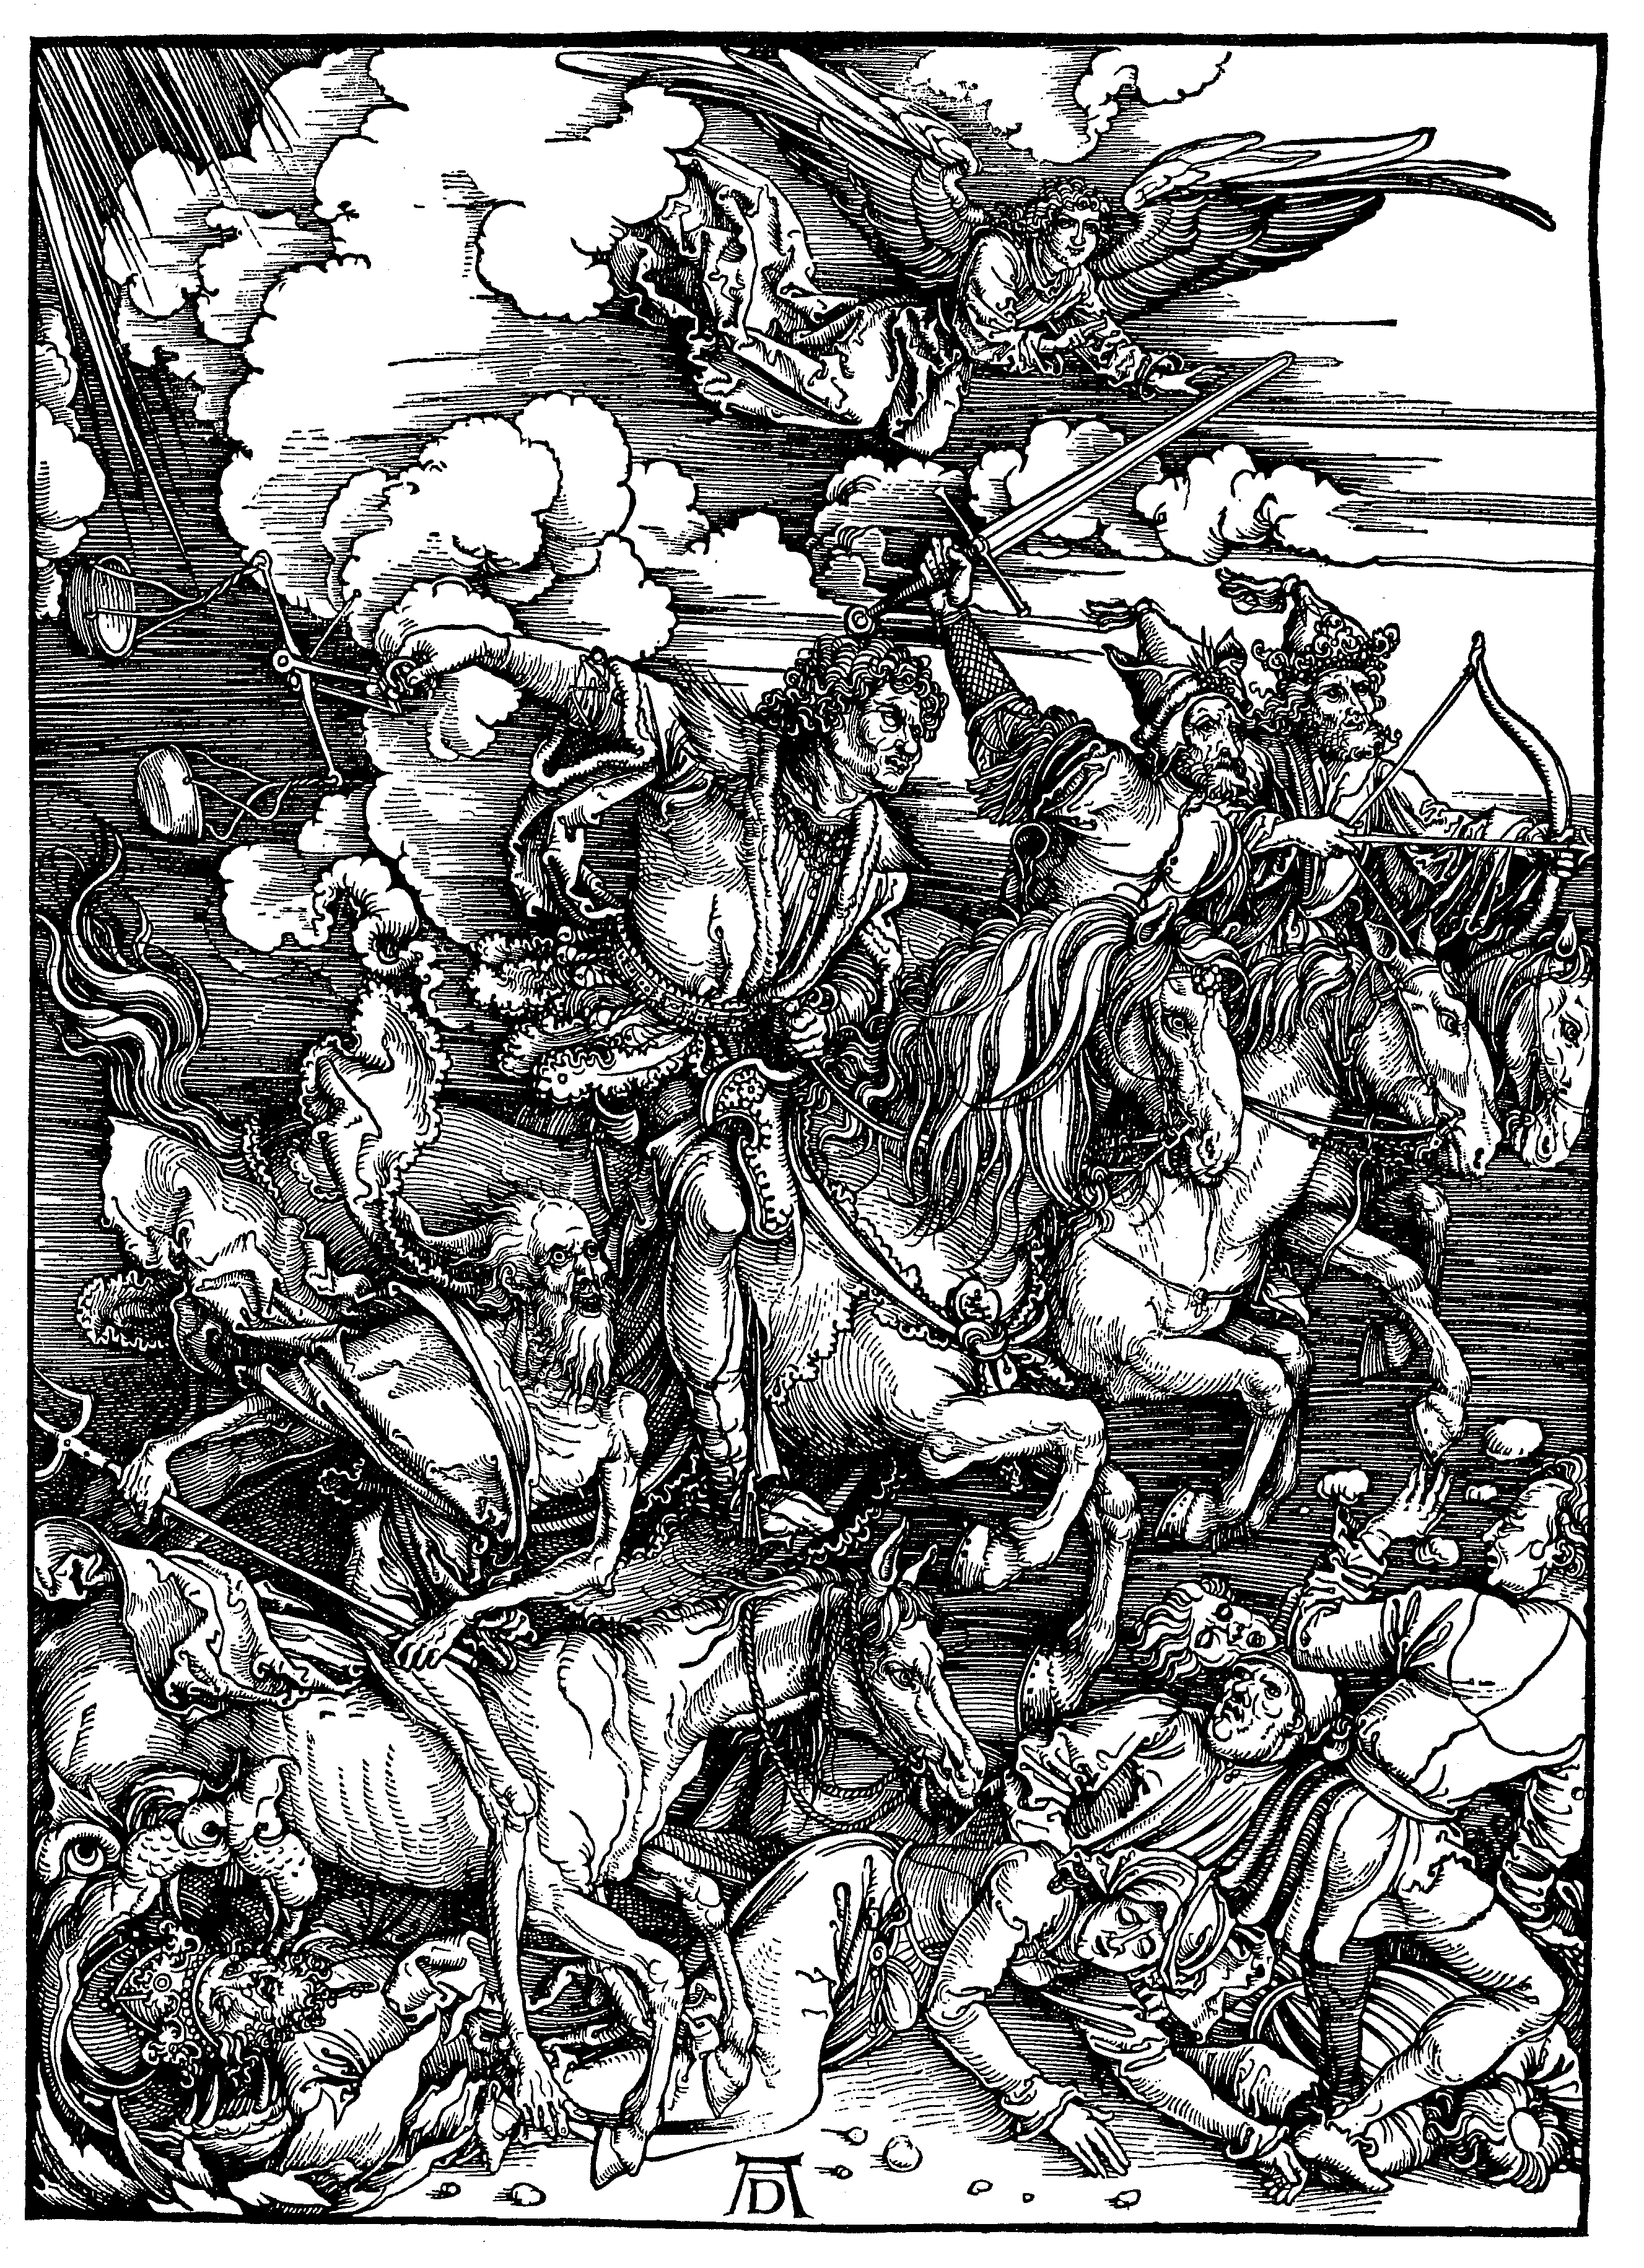
\includegraphics[scale=0.18]{Durer/Durer_Revelation_Four_Riders.jpg}    
    	\caption{La Visión de los Cuatro Jinetes. Albrecht Dürer, 1498.}
\end{figure*}
\chapter{Los Primeros Seis Sellos}
\subsubsection*{El primer sello}
\lettrine[lines=4]{\textcolor{red}{E}}{}ntonces vi cuando el Cordero abrió uno de los siete sellos, y oí a uno de los cuatro seres vivientes que decía, como con voz de trueno: «Ven». \vnum{2} Miré, y había un caballo blanco. El que estaba montado en él tenía un arco. Se le dio una corona, y salió conquistando y para conquistar.
\subsubsection*{El segundo sello}
\vnum{3} Cuando el Cordero abrió el segundo sello, oí al segundo ser viviente que decía: «Ven». \vnum{4} Entonces salió otro caballo, rojo. Al que estaba montado en él se le concedió quitar la paz de la tierra y que los hombres se mataran unos a otros; y se le dio una gran espada.
\subsubsection*{El tercer sello}
\vnum{5} Cuando el Cordero abrió el tercer sello, oí al tercer ser viviente que decía: «Ven». Y miré, y había un caballo negro. El que estaba montado en él tenía una balanza en la mano. \vnum{6} Y oí como una voz en medio de los cuatro seres vivientes que decía: «Un litro de trigo por un denario, y tres litros de cebada por un denario, y no dañes el aceite y el vino».
\subsubsection*{El cuarto sello}
\vnum{7} Cuando el Cordero abrió el cuarto sello, oí la voz del cuarto ser viviente que decía: «Ven». \vnum{8} Y miré, y había un caballo amarillento. El que estaba montado en él se llamaba Muerte, y el Hades lo seguía. Y se les dio autoridad sobre la cuarta parte de la tierra, para matar con espada, con hambre, con pestilencia y con las fieras de la tierra.
\subsubsection*{El quinto sello}
\vnum{9} Cuando el Cordero abrió el quinto sello, vi debajo del altar las almas de los que habían sido muertos a causa de la palabra de Dios y del testimonio que habían mantenido. \vnum{10} Clamaban a gran voz: «¿Hasta cuándo, oh Señor santo y verdadero, esperarás para juzgar y vengar nuestra sangre de los que moran en la tierra?». \vnum{11} Y se les dio a cada uno de ellos una vestidura blanca, y se les dijo que descansaran un poco más de tiempo, hasta que se completara también el número de sus consiervos y de sus hermanos que habrían de ser muertos como ellos lo habían sido.
\subsubsection*{El sexto sello}
\vnum{12} Vi cuando el Cordero abrió el sexto sello, y hubo un gran terremoto, y el sol se puso negro como cilicio hecho de cerda, y toda la luna se volvió como sangre, \vnum{13} y las estrellas del cielo cayeron a la tierra, como la higuera deja caer sus higos verdes al ser sacudida por un fuerte viento. \vnum{14} El cielo desapareció como un pergamino que se enrolla, y todo monte e isla fueron removidos de su lugar.

\vnum{15} Los reyes de la tierra, y los grandes, los comandantes, los ricos, los poderosos, y todo siervo y todo libre, se escondieron en las cuevas y entre las peñas de los montes, \vnum{16} y decían* a los montes y a las peñas: «Caigan sobre nosotros y escóndannos de la presencia de Aquel que está sentado en el trono y de la ira del Cordero. \vnum{17} Porque ha llegado el gran día de la ira de ellos, ¿y quién podrá sostenerse?».
\begin{figure*}[p!]
	\centering
       \includegraphics[scale=0.65]{Durer/Dürer_Apocalypse_5 red.jpg}    
    	\caption{Las Almas Debajo del Altar. Albrecht Dürer, 1498.}
\end{figure*}
\chapter{Los 144,000}
\lettrine[lines=4]{\textcolor{red}{D}}{}espués de esto, vi a cuatro ángeles de pie en los cuatro extremos de la tierra, que detenían los cuatro vientos de la tierra, para que no soplara viento alguno, ni sobre la tierra ni sobre el mar ni sobre ningún árbol. 2 También vi a otro ángel que subía de donde sale el sol y que tenía el sello del Dios vivo. Y gritó a gran voz a los cuatro ángeles a quienes se les había concedido hacer daño a la tierra y al mar: 3 «No hagan daño, ni a la tierra ni al mar ni a los árboles, hasta que hayamos puesto un sello en la frente a los siervos de nuestro Dios».

4 Oí el número de los que fueron sellados: 144,000 sellados de todas las tribus de los israelitas. 5 De la tribu de Judá fueron sellados 12,000; de la tribu de Rubén, 12,000; de la tribu de Gad, 12,000; 6 de la tribu de Aser, 12,000; de la tribu de Neftalí, 12,000; de la tribu de Manasés, 12,000; 7 de la tribu de Simeón, 12,000; de la tribu de Leví, 12,000; de la tribu de Isacar, 12,000; 8 de la tribu de Zabulón, 12,000; de la tribu de José, 12,000 y de la tribu de Benjamín fueron sellados 12,000.
Los redimidos de todas las naciones

9 Después de esto miré, y vi una gran multitud, que nadie podía contar, de todas las naciones, tribus, pueblos, y lenguas, de pie delante del trono y delante del Cordero, vestidos con vestiduras blancas y con palmas en las manos. 10 Clamaban a gran voz:

«La salvación pertenece a nuestro Dios que está sentado en el trono, y al Cordero».

11 Todos los ángeles estaban de pie alrededor del trono y alrededor de los ancianos y de los cuatro seres vivientes. Estos cayeron sobre sus rostros delante del trono y adoraron a Dios,

12 diciendo:

«¡Amén! La bendición, la gloria, la sabiduría, la acción de gracias, el honor, el poder y la fortaleza, sean a nuestro Dios por los siglos de los siglos. Amén».

13 Uno de los ancianos habló diciéndome: «Estos que están vestidos con vestiduras blancas, ¿quiénes son y de dónde han venido?». 14 Y le respondí: «Señor mío, usted lo sabe». Y él me dijo: «Estos son los que vienen de la gran tribulación, y han lavado sus vestiduras y las han emblanquecido en la sangre del Cordero. 15 Por eso están delante del trono de Dios, y le sirven día y noche en Su templo; y Aquel que está sentado en el trono extenderá Su tabernáculo sobre ellos. 16 Ya no tendrán hambre ni sed, ni el sol les hará daño, ni ningún calor abrasador, 17 pues el Cordero que está en medio del trono los pastoreará y los guiará a manantiales de aguas de vida, y Dios enjugará toda lágrima de sus ojos».
\begin{figure*}[p!]
	\centering
       \includegraphics[scale=0.5]{Durer/Dürer_Apocalypse_6.jpg}    
    	\caption{La Visión de los 144,000. Albrecht Dürer, 1498.}
\end{figure*}
\chapter{}
\lettrine[lines=4]{\textcolor{red}{C}}{}uando el Cordero abrió el séptimo sello, hubo silencio en el cielo como por media hora. 2 Vi a los siete ángeles que están de pie delante de Dios, y se les dieron siete trompetas.

3 Otro ángel vino y se paró ante el altar con un incensario de oro, y se le dio mucho incienso para que lo añadiera a las oraciones de todos los santos sobre el altar de oro que estaba delante del trono. 4 De la mano del ángel subió ante Dios el humo del incienso con las oraciones de los santos. 5 Después el ángel tomó el incensario, lo llenó con el fuego del altar y lo arrojó a la tierra, y hubo truenos, ruidos, relámpagos, y un terremoto.
Las primeras cuatro trompetas

6 Entonces los siete ángeles que tenían las siete trompetas se prepararon para tocarlas.

7 El primero tocó la trompeta, y vino granizo y fuego mezclados con sangre, y fueron arrojados a la tierra. Se quemó la tercera parte de la tierra, la tercera parte de los árboles y toda hierba verde.

8 El segundo ángel tocó la trompeta, y algo como una gran montaña ardiendo en llamas fue arrojado al mar, y la tercera parte del mar se convirtió en sangre. 9 Y murió la tercera parte de los seres que estaban en el mar y que tenían vida. Y la tercera parte de los barcos fue destruida.

10 El tercer ángel tocó la trompeta, y cayó del cielo una gran estrella, ardiendo como una antorcha, y cayó sobre la tercera parte de los ríos y sobre los manantiales de las aguas. 11 El nombre de la estrella es Ajenjo. La tercera parte de las aguas se convirtió en ajenjo, y muchos hombres murieron por causa de las aguas, porque se habían vuelto amargas.

12 El cuarto ángel tocó la trompeta, y fue herida la tercera parte del sol, la tercera parte de la luna, y la tercera parte de las estrellas, para que la tercera parte de ellos se oscureciera y el día no resplandeciera en su tercera parte, y asimismo en la noche.

13 Entonces miré, y oí volar un águila en medio del cielo, que decía a gran voz: «¡Ay, ay, ay, de los que habitan en la tierra, a causa de los toques de trompeta que faltan, que los otros tres ángeles están para tocar!».
\begin{figure*}[p!]
	\centering
       \includegraphics[scale=0.5]{Durer/Dürer_Apocalypse_7.jpg}    
    	\caption{La Visión de San Juan de los Siete Candelabros. Albrecht Dürer, 1498.}
\end{figure*}
\chapter{}
\lettrine[lines=4]{\textcolor{red}{E}}{}l quinto ángel tocó la trompeta, y vi una estrella que había caído del cielo a la tierra, y se le dio la llave del pozo del abismo. 2 Cuando abrió el pozo del abismo, subió humo del pozo como el humo de un gran horno, y el sol y el aire se oscurecieron por el humo del pozo. 3 Del humo salieron langostas sobre la tierra, y se les dio poder como tienen poder los escorpiones de la tierra.

4 Se les dijo que no dañaran la hierba de la tierra, ni ninguna cosa verde, ni ningún árbol, sino solo a los hombres que no tienen el sello de Dios en la frente. 5 No se les permitió matar a nadie, sino atormentarlos por cinco meses. Su tormento era como el tormento de un escorpión cuando pica al hombre. 6 En aquellos días los hombres buscarán la muerte y no la hallarán; y ansiarán morir, y la muerte huirá de ellos.

7 El aspecto de las langostas era semejante al de caballos dispuestos para la batalla, y sobre sus cabezas tenían como coronas que parecían de oro, y sus caras eran como rostros humanos. 8 Tenían cabellos como cabellos de mujer, y sus dientes eran como de leones. 9 También tenían corazas como corazas de hierro. El ruido de sus alas era como el estruendo de carros, de muchos caballos que se lanzan a la batalla. 10 Tienen colas parecidas a escorpiones, y aguijones. En sus colas está su poder para hacer daño a los hombres por cinco meses. 11 Tienen sobre ellos por rey al ángel del abismo, cuyo nombre en hebreo es Abadón, y en griego se llama Apolión.

12 El primer ¡ay! ha pasado; pero aún vienen dos ayes después de estas cosas.
La sexta trompeta

13 El sexto ángel tocó la trompeta, y oí una voz que salía de los cuatro cuernos del altar de oro que está delante de Dios, 14 y decía al sexto ángel que tenía la trompeta: «Suelta a los cuatro ángeles que están atados junto al gran río Éufrates». 15 Y fueron desatados los cuatro ángeles que habían sido preparados para la hora, el día, el mes, y el año, para matar a la tercera parte de la humanidad.

16 El número de los ejércitos de los jinetes era doscientos millones; yo escuché su número. 17 Así es como vi en la visión los caballos y a los que los montaban: los jinetes tenían corazas color de fuego, de jacinto y de azufre. Las cabezas de los caballos eran como cabezas de leones, y de sus bocas salía fuego, humo, y azufre.

18 La tercera parte de la humanidad fue muerta por estas tres plagas: por el fuego, el humo, y el azufre que salían de sus bocas. 19 Porque el poder de los caballos está en su boca y en sus colas; pues sus colas son semejantes a serpientes, tienen cabezas y con ellas hacen daño.

20 El resto de la humanidad, los que no fueron muertos por estas plagas, no se arrepintieron de las obras de sus manos ni dejaron de adorar a los demonios y a los ídolos de oro, de plata, de bronce, de piedra, y de madera, que no pueden ver ni oír ni andar. 21 Tampoco se arrepintieron de sus homicidios ni de sus hechicerías ni de su inmoralidad ni de sus robos.
\begin{figure*}[p!]
	\centering
       \includegraphics[scale=0.5]{Durer/Dürer_Apocalypse_8.jpg}    
    	\caption{La Visión de San Juan de los Siete Candelabros. Albrecht Dürer, 1498.}
\end{figure*}
\chapter{}
\lettrine[lines=4,slope=-.5em]{\textcolor{red}{V}}{\ }i a otro ángel poderoso que descendía del cielo, envuelto en una nube. El arco iris estaba sobre su cabeza, su rostro era como el sol y sus pies como columnas de fuego. 2 Tenía en su mano un librito abierto. Puso el pie derecho sobre el mar y el izquierdo sobre la tierra, 3 y gritó a gran voz, como ruge un león. Y cuando gritó, los siete truenos emitieron sus voces. 4 Después que los siete truenos hablaron, iba yo a escribir, cuando oí una voz del cielo que decía: «Sella las cosas que los siete truenos han dicho y no las escribas».

5 Entonces el ángel que yo había visto de pie sobre el mar y sobre la tierra, levantó su mano derecha al cielo, 6 y juró por Aquel que vive por los siglos de los siglos, quien creó el cielo y las cosas que en Él hay, y la tierra y las cosas que en ella hay, y el mar y las cosas que en Él hay, que ya no habrá más demora. 7 Porque en los días de la voz del séptimo ángel, cuando esté para tocar la trompeta, entonces el misterio de Dios será consumado, como Él lo anunció a Sus siervos los profetas.

8 La voz que yo había oído del cielo, la oí de nuevo hablando conmigo: «Ve, toma el libro que está abierto en la mano del ángel que está de pie sobre el mar y sobre la tierra». 9 Entonces fui al ángel y le dije que me diera el librito. Y él me dijo*: «Tómalo y devóralo. Te amargará las entrañas, pero en tu boca será dulce como la miel». 10 Tomé el librito de la mano del ángel y lo devoré, y en mi boca fue dulce como la miel; pero cuando lo comí, me amargó las entrañas.

11 Y me dijeron*: «Debes profetizar otra vez acerca de muchos pueblos, naciones, lenguas y reyes».
\chapter{}
\lettrine[lines=4]{\textcolor{red}{M}}{}e fue dada una caña de medir (unos 3 metros) semejante a una vara, y alguien dijo: «Levántate y mide el templo de Dios y el altar, y a los que en él adoran. 2 Pero excluye el patio que está fuera del templo, no lo midas, porque ha sido entregado a las naciones, y estas pisotearán la ciudad santa por cuarenta y dos meses.

3 »Otorgaré autoridad a mis dos testigos, y ellos profetizarán por 1,260 días, vestidos de cilicio». 4 Estos son los dos olivos y los dos candelabros que están delante del Señor de la tierra. 5 Si alguien quiere hacerles daño, de su boca sale fuego y devora a sus enemigos. Así debe morir cualquiera que quisiera hacerles daño. 6 Ellos tienen poder para cerrar el cielo a fin de que no llueva durante los días en que ellos profeticen; y tienen poder sobre las aguas para convertirlas en sangre, y para herir la tierra con toda suerte de plagas todas las veces que quieran.

7 Cuando hayan terminado de dar su testimonio, la bestia que sube del abismo hará guerra contra ellos, los vencerá y los matará. 8 Sus cadáveres estarán en la calle de la gran ciudad, que simbólicamente se llama Sodoma y Egipto, donde también su Señor fue crucificado. 9 Gente de todos los pueblos, tribus, lenguas, y naciones, contemplarán sus cadáveres por tres días y medio, y no permitirán que sus cadáveres sean sepultados. 10 Los que moran en la tierra se regocijarán por ellos y se alegrarán, y se enviarán regalos unos a otros, porque estos dos profetas habían atormentado a los que moran en la tierra.

11 Pero después de los tres días y medio, el aliento de vida de parte de Dios vino a ellos y se pusieron en pie, y gran temor cayó sobre quienes los contemplaban. 12 Entonces ellos oyeron una gran voz del cielo que les decía: «Suban acá». Y subieron al cielo en la nube, y sus enemigos los vieron.

13 En aquella misma hora hubo un gran terremoto y la décima parte de la ciudad se derrumbó, y siete mil personas murieron en el terremoto, y los demás, aterrorizados, dieron gloria al Dios del cielo.

14 El segundo ¡ay! ha pasado; pero el tercer ¡ay! viene pronto.
La séptima trompeta

15 El séptimo ángel tocó la trompeta, y hubo grandes voces en el cielo, que decían:

«El reino del mundo ha venido a ser el reino de nuestro Señor y de Su Cristo. Él reinará por los siglos de los siglos». 16 Y los veinticuatro ancianos que estaban sentados delante de Dios en sus tronos, se postraron sobre sus rostros y adoraron a Dios, 17 diciendo:

«Te damos gracias, oh Señor Dios Todopoderoso, el que eres y el que eras, porque has tomado Tu gran poder y has comenzado a reinar. 18 Las naciones se enfurecieron, y vino Tu ira y llegó el tiempo de juzgar a los muertos y de dar la recompensa a Tus siervos los profetas, a los santos y a los que temen Tu nombre, a los pequeños y a los grandes, y de destruir a los que destruyen la tierra».

19 El templo de Dios que está en el cielo fue abierto; y el arca de Su pacto se veía en Su templo, y hubo relámpagos, voces y truenos, y un terremoto y una fuerte granizada.
\chapter{}
\lettrine[lines=4]{\textcolor{red}{U}}{\ }na gran señal apareció en el cielo: una mujer vestida del sol, con la luna debajo de sus pies, y una corona de doce estrellas sobre su cabeza. 2 Estaba encinta, y gritaba* por los dolores del parto y el sufrimiento de dar a luz.

3 Entonces apareció otra señal en el cielo: Un gran dragón rojo que tenía siete cabezas y diez cuernos, y sobre sus cabezas había siete diademas. 4 Su cola arrastró* la tercera parte de las estrellas del cielo y las arrojó sobre la tierra. Y el dragón se paró delante de la mujer que estaba para dar a luz, a fin de devorar a su hijo cuando ella diera a luz. 5 Y ella dio a luz un Hijo varón, que ha de regir a todas las naciones con vara de hierro. Su Hijo fue arrebatado hasta Dios y hasta Su trono. 6 La mujer huyó al desierto, donde tenía* un lugar preparado por Dios, para ser sustentada allí por 1,260 días.

7 Entonces hubo guerra en el cielo: Miguel y sus ángeles combatieron contra el dragón. Y el dragón y sus ángeles lucharon, 8 pero no pudieron vencer, ni se halló ya lugar para ellos en el cielo. 9 Y fue arrojado el gran dragón, la serpiente antigua que se llama Diablo y Satanás, el cual engaña al mundo entero. Fue arrojado a la tierra y sus ángeles fueron arrojados con él.

10 Entonces oí una gran voz en el cielo, que decía:

«Ahora ha venido la salvación, el poder y el reino de nuestro Dios y la autoridad de Su Cristo, porque el acusador de nuestros hermanos, el que los acusa delante de nuestro Dios día y noche, ha sido arrojado. 11 Ellos lo vencieron por medio de la sangre del Cordero y por la palabra del testimonio de ellos, y no amaron sus vidas, llegando hasta sufrir la muerte. 12 Por lo cual regocíjense, cielos y los que moran en ellos. ¡Ay de la tierra y del mar!, porque el diablo ha descendido a ustedes con gran furor, sabiendo que tiene poco tiempo».

13 Cuando el dragón vio que había sido arrojado a la tierra, persiguió a la mujer que había dado a luz al Hijo varón. 14 Y se le dieron a la mujer las dos alas de la gran águila a fin de que volara de la presencia de la serpiente al desierto, a su lugar, donde fue* sustentada por un tiempo, tiempos y medio tiempo. 15 La serpiente arrojó de su boca, tras la mujer, agua como un río, para que ella fuera arrastrada por la corriente.

16 Pero la tierra ayudó a la mujer, y la tierra abrió su boca y tragó el río que el dragón había arrojado de su boca. 17 Entonces el dragón se enfureció contra la mujer, y salió para hacer guerra contra el resto de la descendencia de ella, los que guardan los mandamientos de Dios y tienen el testimonio de Jesús.
\chapter{}
\lettrine[lines=4]{\textcolor{red}{E}}{}l dragón se paró sobre la arena del mar.

\zz Y vi que subía del mar una bestia que tenía diez cuernos y siete cabezas. En sus cuernos había diez diademas, y en sus cabezas había nombres blasfemos. 2 La bestia que vi era semejante a un leopardo, sus pies eran como los de un oso y su boca como la boca de un león. El dragón le dio su poder, su trono, y gran autoridad. 3 Vi una de sus cabezas como herida de muerte, pero su herida mortal fue sanada. Y la tierra entera se maravilló y seguía tras la bestia. 4 Adoraron al dragón, porque había dado autoridad a la bestia. Adoraron a la bestia, diciendo: «¿Quién es semejante a la bestia, y quién puede luchar contra ella?».

5 A la bestia se le dio una boca que hablaba palabras arrogantes y blasfemias, y se le dio autoridad para actuar durante cuarenta y dos meses. 6 Y abrió su boca con blasfemias contra Dios, para blasfemar Su nombre y Su tabernáculo, es decir, contra los que moran en el cielo. 7 Se le concedió hacer guerra contra los santos y vencerlos. Y se le dio autoridad sobre toda tribu, pueblo, lengua y nación. 8 Adorarán a la bestia todos los que moran en la tierra, cuyos nombres no han sido escritos desde la fundación del mundo en el libro de la vida del Cordero que fue inmolado.

9 Si alguno tiene oído, que oiga. 10 Si alguien es destinado a la cautividad, a la cautividad va; si alguien ha de morir a espada, a espada ha de morir. Aquí está la perseverancia y la fe de los santos.
La bestia que sube de la tierra

11 Vi otra bestia que subía de la tierra. Tenía dos cuernos semejantes a los de un cordero y hablaba como un dragón. 12 Ejerce toda la autoridad de la primera bestia en su presencia, y hace que la tierra y los que moran en ella adoren a la primera bestia, cuya herida mortal fue sanada. 13 También hace grandes señales, de tal manera que aun hace descender fuego del cielo a la tierra en presencia de los hombres. 14 Además engaña a los que moran en la tierra a causa de las señales que se le concedió hacer en presencia de la bestia, diciendo a los moradores de la tierra que hagan una imagen de la bestia que tenía* la herida de la espada y que ha vuelto a vivir.

15 Se le concedió dar aliento a la imagen de la bestia, para que la imagen de la bestia también hablara y diera muerte a todos los que no adoran la imagen de la bestia. 16 Y hace que a todos, pequeños y grandes, ricos y pobres, libres y esclavos, se les dé una marca en la mano derecha o en la frente, 17 para que nadie pueda comprar ni vender, sino el que tenga la marca, la cual es el nombre de la bestia o el número de su nombre.

18 Aquí hay sabiduría. El que tiene entendimiento, que calcule el número de la bestia, porque el número es el de un hombre, y su número es 666.
\chapter{}
\lettrine[lines=4]{\textcolor{red}{M}}{}iré que el Cordero estaba de pie sobre el monte Sión, y con Él 144,000 que tenían el nombre del Cordero y el nombre de Su Padre escrito en la frente. 2 Oí una voz del cielo, como el estruendo de muchas aguas y como el sonido de un gran trueno. La voz que oí era como el sonido de arpistas tocando sus arpas. 3 Y cantaban* un cántico nuevo delante del trono y delante de los cuatro seres vivientes y de los ancianos. Nadie podía aprender el cántico, sino los 144,000 que habían sido rescatados de la tierra.

4 Estos son los que no se han contaminado con mujeres, pues son castos. Estos son los que siguen al Cordero adondequiera que va. Estos han sido rescatados de entre los hombres como primicias para Dios y para el Cordero. 5 En su boca no fue hallado engaño; están sin mancha.
El mensaje de los tres ángeles

6 Después vi volar en medio del cielo a otro ángel que tenía un evangelio eterno para anunciarlo a los que moran en la tierra, y a toda nación, tribu, lengua, y pueblo, 7 que decía a gran voz: «Teman a Dios y den a Él gloria, porque la hora de Su juicio ha llegado. Adoren al que hizo el cielo y la tierra, el mar y las fuentes de las aguas».

8 Lo siguió otro ángel, el segundo, diciendo: «¡Cayó, cayó la gran Babilonia!, la que ha hecho beber a todas las naciones del vino de la pasión de su inmoralidad».

9 Entonces los siguió otro ángel, el tercero, diciendo a gran voz: «Si alguien adora a la bestia y a su imagen, y recibe una marca en su frente o en su mano, 10 él también beberá del vino del furor de Dios, que está preparado puro en la copa de Su ira. Será atormentado con fuego y azufre delante de los santos ángeles y en presencia del Cordero. 11 El humo de su tormento asciende por los siglos de los siglos. No tienen reposo, ni de día ni de noche, los que adoran a la bestia y a su imagen, y cualquiera que reciba la marca de su nombre». 12 Aquí está la perseverancia de los santos que guardan los mandamientos de Dios y la fe de Jesús.

13 Entonces oí una voz del cielo que decía: «Escribe: “Bienaventurados los muertos que de aquí en adelante mueren en el Señor”». «Sí», dice el Espíritu, «para que descansen de sus trabajos, porque sus obras van con ellos».
La siega de la tierra

14 Y miré, y había una nube blanca, y en la nube estaba sentado uno semejante al Hijo del Hombre, que tenía en la cabeza una corona de oro, y en la mano una hoz afilada. 15 Entonces salió del templo otro ángel clamando a gran voz a Aquel que estaba sentado en la nube: «Mete Tu hoz y siega, porque la hora de segar ha llegado, pues la cosecha de la tierra está madura». 16 Aquel que estaba sentado en la nube metió Su hoz sobre la tierra y la tierra fue segada.

17 Otro ángel salió del templo que está en el cielo, que también tenía una hoz afilada. 18 Entonces otro ángel, el que tiene poder sobre el fuego, salió del altar, y llamó con gran voz al que tenía la hoz afilada, diciéndole: «Mete tu hoz afilada y vendimia los racimos de la vid de la tierra, porque sus uvas están maduras». 19 El ángel metió su hoz sobre la tierra, y vendimió los racimos de la vid de la tierra y los echó en el gran lagar del furor de Dios. 20 El lagar fue pisado fuera de la ciudad, y del lagar salió sangre que subió hasta los frenos de los caballos por una distancia como de 320 kilómetros.
\chapter{}
\lettrine[lines=4]{\textcolor{red}{E}}{}ntonces vi otra señal en el cielo, grande y maravillosa: siete ángeles que tenían siete plagas, las últimas, porque en ellas se ha consumado el furor de Dios.

2 Vi también como un mar de cristal mezclado con fuego, y a los que habían salido victoriosos sobre la bestia, sobre su imagen y sobre el número de su nombre, en pie sobre el mar de cristal, con arpas de Dios. 3 Y cantaban* el cántico de Moisés, siervo de Dios, y el cántico del Cordero, diciendo:

«¡Grandes y maravillosas son Tus obras, oh Señor Dios, Todopoderoso!
¡Justos y verdaderos son Tus caminos, oh Rey de las naciones!
4 
¡Oh Señor! ¿Quién no temerá y glorificará Tu nombre?
Pues solo Tú eres santo;
Porque todas las naciones vendrán
Y adorarán en Tu presencia,
Pues Tus justos juicios han sido revelados».

5 Después de estas cosas miré, y se abrió el templo del tabernáculo del testimonio en el cielo. 6 Y salieron del templo los siete ángeles que tenían las siete plagas. Estaban vestidos de lino puro y resplandeciente, y ceñidos alrededor del pecho con cintos de oro. 7 Entonces uno de los cuatro seres vivientes dio a los siete ángeles siete copas de oro llenas del furor de Dios, quien vive por los siglos de los siglos. 8 El templo se llenó del humo de la gloria de Dios y de Su poder. Nadie podía entrar al templo hasta que se terminaran las siete plagas de los siete ángeles.
\chapter{}
\lettrine[lines=4]{\textcolor{red}{O}}{}í entonces una gran voz que desde el templo decía a los siete ángeles: «Vayan y derramen en la tierra las siete copas del furor de Dios».

2 El primer ángel fue y derramó su copa en la tierra, y se produjo una llaga repugnante y maligna en los hombres que tenían la marca de la bestia y que adoraban su imagen.

3 El segundo ángel derramó su copa en el mar, y se convirtió en sangre como de muerto; y murió todo ser viviente que había en el mar.

4 El tercer ángel derramó su copa en los ríos y en las fuentes de las aguas, y se convirtieron en sangre. 5 Oí al ángel de las aguas, que decía: «Justo eres Tú, el que eres, y el que eras, oh Santo, porque has juzgado estas cosas; 6 pues ellos derramaron sangre de santos y profetas y Tú les has dado a beber sangre. Se lo merecen». 7 También oí al altar, que decía: «Sí, oh Señor Dios Todopoderoso, verdaderos y justos son Tus juicios».

8 El cuarto ángel derramó su copa sobre el sol. Y al sol se le permitió quemar a los hombres con fuego. 9 Y los hombres fueron quemados con el intenso calor. Blasfemaron el nombre de Dios que tiene poder sobre estas plagas, y no se arrepintieron para darle gloria a Él.

10 El quinto ángel derramó su copa sobre el trono de la bestia, y su reino se quedó en tinieblas; y todos se mordían la lengua de dolor. 11 Blasfemaron contra el Dios del cielo por causa de sus dolores y de sus llagas, y no se arrepintieron de sus obras.

12 El sexto ángel derramó su copa sobre el gran Río Éufrates; y sus aguas se secaron para que fuera preparado el camino para los reyes del oriente. 13 Y vi salir de la boca del dragón, de la boca de la bestia, y de la boca del falso profeta, a tres espíritus inmundos semejantes a ranas. 14 Pues son espíritus de demonios que hacen señales, los cuales van a los reyes de todo el mundo, a reunirlos para la batalla del gran día del Dios Todopoderoso.

15 «¡Estén alerta! Vengo como ladrón. Bienaventurado el que vela y guarda sus ropas, no sea que ande desnudo y vean su vergüenza». 16 Entonces los reunieron en el lugar que en hebreo se llama Armagedón.

17 El séptimo ángel derramó su copa en el aire. Una gran voz salió del templo, del trono, que decía: «Hecho está». 18 Y hubo relámpagos, voces, y truenos. Hubo un gran terremoto tal como no lo había habido desde que el hombre está sobre la tierra; fue tan grande y poderoso el terremoto. 19 La gran ciudad quedó dividida en tres partes, y las ciudades de las naciones cayeron. Y la gran Babilonia fue recordada delante de Dios para darle la copa del vino del furor de Su ira. 20 Entonces toda isla huyó y los montes no fueron hallados. 21 Enormes granizos, como de 45 kilos cada uno, cayeron* sobre los hombres. Y los hombres blasfemaron contra Dios por la plaga del granizo, porque esa plaga fue* sumamente grande.
\chapter{}
\lettrine[lines=4]{\textcolor{red}{U}}{\ }no de los siete ángeles que tenían las siete copas, vino y habló conmigo: «Ven; te mostraré el juicio de la gran ramera que está sentada sobre muchas aguas. 2 Con ella los reyes de la tierra cometieron actos inmorales, y los moradores de la tierra fueron embriagados con el vino de su inmoralidad».

3 Entonces me llevó en el Espíritu a un desierto. Vi a una mujer sentada sobre una bestia escarlata, llena de nombres blasfemos, y que tenía siete cabezas y diez cuernos. 4 La mujer estaba vestida de púrpura y escarlata, y adornada con oro, y piedras preciosas, y perlas. Tenía en la mano una copa de oro llena de abominaciones y de las inmundicias de su inmoralidad. 5 Sobre su frente había un nombre escrito, un misterio: «BABILONIA LA GRANDE, LA MADRE DE LAS RAMERAS Y DE LAS ABOMINACIONES DE LA TIERRA». 6 Vi a la mujer ebria de la sangre de los santos, y de la sangre de los testigos de Jesús. Al verla, me asombré grandemente.

7 Y el ángel me dijo: «¿Por qué te has asombrado? Yo te diré el misterio de la mujer y de la bestia que la lleva, la que tiene las siete cabezas y los diez cuernos. 8 La bestia que viste, era y ya no existe, y está para subir del abismo e ir a la destrucción. Y los moradores de la tierra, cuyos nombres no se han escrito en el libro de la vida desde la fundación del mundo, se asombrarán al ver la bestia que era y ya no existe, pero que vendrá.

9 »Aquí está la mente que tiene sabiduría. Las siete cabezas son siete montes sobre los que se sienta la mujer. 10 También son siete reyes: cinco han caído, uno es y el otro aún no ha venido; y cuando venga, es necesario que permanezca un poco de tiempo. 11 Y la bestia que era y ya no existe, es el octavo rey, y es uno de los siete y va a la destrucción. 12 Los diez cuernos que viste son diez reyes que todavía no han recibido reino, pero que por una hora reciben autoridad como reyes con la bestia. 13 Estos tienen un mismo propósito, y entregarán su poder y autoridad a la bestia. 14 Ellos pelearán contra el Cordero, pero el Cordero los vencerá, porque Él es Señor de señores y Rey de reyes, y los que están con Él son llamados, escogidos y fieles».

15 También el ángel me dijo*: «Las aguas que viste donde se sienta la ramera, son pueblos, multitudes, naciones y lenguas. 16 Y los diez cuernos que viste y la bestia odiarán a la ramera y la dejarán desolada y desnuda, y comerán sus carnes y la quemarán con fuego. 17 Porque Dios ha puesto en sus corazones el ejecutar Su propósito: que tengan ellos un propósito unánime, y den su reino a la bestia hasta que las palabras de Dios se cumplan. 18 La mujer que viste es la gran ciudad, que reina sobre los reyes de la tierra».
\chapter{}
\lettrine[lines=4]{\textcolor{red}{D}}{}espués de esto vi a otro ángel descender del cielo, que tenía gran poder, y la tierra fue iluminada con su gloria. 2 Y gritó con potente voz: «¡Cayó, cayó la gran Babilonia! Se ha convertido en habitación de demonios, en guarida de todo espíritu inmundo y en guarida de toda ave inmunda y aborrecible. 3 Porque todas las naciones han bebido del vino de la pasión de su inmoralidad, y los reyes de la tierra han cometido actos inmorales con ella, y los mercaderes de la tierra se han enriquecido con la riqueza de su sensualidad».

4 Y oí otra voz del cielo que decía: «Salgan de ella, pueblo mío, para que no participen de sus pecados y para que no reciban de sus plagas. 5 Porque sus pecados se han amontonado hasta el cielo, y Dios se ha acordado de sus iniquidades. 6 Páguenle tal como ella ha pagado, y devuélvanle doble según sus obras. En la copa que ella ha preparado, preparen el doble para ella. 7 Cuanto ella se glorificó a sí misma y vivió sensualmente, así denle tormento y duelo, porque dice en su corazón: “Yo estoy sentada como reina, y no soy viuda y nunca veré duelo”.

8 »Por eso, en un solo día, vendrán sus plagas: muerte, duelo, y hambre, y será quemada con fuego; porque el Señor Dios que la juzga es poderoso. 9 Y los reyes de la tierra que cometieron actos de inmoralidad y vivieron sensualmente con ella, llorarán y se lamentarán por ella cuando vean el humo de su incendio. 10 Y de pie, desde lejos por causa del temor de su tormento, dirán: “¡Ay, ay, la gran ciudad, Babilonia, la ciudad fuerte! Porque en una hora ha llegado tu juicio”.

11 »Los mercaderes de la tierra lloran y se lamentan por ella, porque ya nadie compra sus mercaderías: 12 cargamentos de oro, plata, piedras preciosas, perlas, lino fino, púrpura, seda y escarlata; toda clase de maderas olorosas y todo objeto de marfil y todo objeto hecho de maderas preciosas, bronce, hierro, y mármol; 13 y canela, especias aromáticas, incienso, perfume, mirra, vino, aceite de oliva; y flor de harina, trigo, bestias, ovejas, caballos, carros, esclavos, y vidas humanas. 14 Y el fruto que tanto has anhelado se ha apartado de ti, y todas las cosas que eran lujosas y espléndidas se han alejado de ti, y nunca más las hallarán. 15 Los mercaderes de estas cosas que se enriquecieron a costa de ella, se pararán lejos a causa del temor de su tormento, llorando y lamentándose, 16 y diciendo: “¡Ay, ay, la gran ciudad, que estaba vestida de lino fino, púrpura y escarlata, y adornada de oro, piedras preciosas y perlas! 17 En una hora ha sido arrasada tanta riqueza”. Todos los capitanes, pasajeros, y marineros, y todos los que viven del mar, se pararon a lo lejos, 18 y al ver el humo de su incendio gritaban: “¿Qué ciudad es semejante a la gran ciudad?”. 19 Y echaron polvo sobre sus cabezas, y llorando y lamentándose, gritaban: “¡Ay, ay, la gran ciudad en la cual todos los que tenían naves en el mar se enriquecieron a costa de sus riquezas!, porque en una hora ha sido asolada”.

20 »Regocíjate sobre ella, cielo, y también ustedes, santos, apóstoles y profetas, porque Dios ha pronunciado juicio contra ella por ustedes».

21 Entonces un ángel poderoso tomó una piedra, como una gran piedra de molino, y la arrojó al mar, diciendo: «Así será derribada con violencia Babilonia, la gran ciudad, y nunca más será hallada. 22 El sonido de arpistas, de músicos, de flautistas, y de trompeteros no se oirá más en ti. Ningún artífice de oficio alguno se hallará más en ti. Ningún ruido de molino se oirá más en ti. 23 Ninguna luz de la lámpara alumbrará más en ti. Tampoco la voz del novio y de la novia se oirá más en ti, porque tus mercaderes eran los grandes de la tierra, pues todas las naciones fueron engañadas por tus hechicerías.

24 »Y en ella fue hallada la sangre de los profetas, de los santos y de todos los que habían sido muertos sobre la tierra».
\chapter{}
\lettrine[lines=4]{\textcolor{red}{D}}{}espués de esto oí como una gran voz de una gran multitud en el cielo, que decía:

\zz«¡Aleluya!
La salvación y la gloria y el poder pertenecen a nuestro Dios,
2 
Porque Sus juicios son verdaderos y justos,
Pues ha juzgado a la gran ramera
Que corrompía la tierra con su inmoralidad,
Y ha vengado la sangre de Sus siervos en ella».

3 Y dijeron por segunda vez:

«¡Aleluya!
El humo de ella sube por los siglos de los siglos».

4 Entonces los veinticuatro ancianos y los cuatro seres vivientes se postraron y adoraron a Dios, que está sentado en el trono, y decían:

«¡Amén! ¡Aleluya!».

5 Y del trono salió una voz que decía:

«Alaben ustedes a nuestro Dios, todos ustedes Sus siervos,
Los que le temen, los pequeños y los grandes».
Anuncio de las bodas del Cordero

6 Oí como la voz de una gran multitud, como el estruendo de muchas aguas y como el sonido de fuertes truenos, que decía:

«¡Aleluya!
Porque el Señor nuestro Dios Todopoderoso reina.
7 
Regocijémonos y alegrémonos, y démosle a Él la gloria,
Porque las bodas del Cordero han llegado y Su esposa se ha preparado».
8 
Y a ella le fue concedido vestirse de lino fino, resplandeciente y limpio,
Porque las acciones justas de los santos son el lino fino.

9 El ángel me dijo*: «Escribe: “Bienaventurados los que están invitados a la cena de las Bodas del Cordero”». También me dijo*: «Estas son palabras verdaderas de Dios». 10 Entonces caí a sus pies para adorarlo. Y me dijo*: «No hagas eso. Yo soy consiervo tuyo y de tus hermanos que poseen el testimonio de Jesús; adora a Dios. El testimonio de Jesús es el espíritu de la profecía».
El jinete del caballo blanco

11 Vi el cielo abierto, y apareció un caballo blanco. El que lo montaba se llama Fiel y Verdadero. Con justicia juzga y hace la guerra. 12 Sus ojos son una llama de fuego, y sobre Su cabeza hay muchas diademas. Tiene un nombre escrito que nadie conoce sino Él. 13 Está vestido de un manto empapado en sangre, y Su nombre es: El Verbo de Dios.

14 Los ejércitos que están en los cielos, vestidos de lino fino, blanco y limpio, lo seguían sobre caballos blancos. 15 De Su boca sale una espada afilada para herir con ella a las naciones y las regirá con vara de hierro. Él mismo pisa el lagar del vino del furor de la ira de Dios Todopoderoso. 16 En Su manto y en Su muslo tiene un nombre escrito: «REY DE REYES Y SEÑOR DE SEÑORES».

17 Vi a un ángel que estaba de pie en el sol. Clamó a gran voz, diciendo a todas las aves que vuelan en medio del cielo: «Vengan, congréguense para la gran cena de Dios, 18 para que coman carne de reyes, carne de comandantes y carne de poderosos, carne de caballos y de sus jinetes, y carne de todos los hombres, libres y esclavos, pequeños y grandes».

19 Entonces vi a la bestia, a los reyes de la tierra y a sus ejércitos reunidos para hacer guerra contra Aquel que iba montado en el caballo blanco y contra Su ejército. 20 Y la bestia fue apresada, junto con el falso profeta que hacía señales en su presencia, con las cuales engañaba a los que habían recibido la marca de la bestia y a los que adoraban su imagen. Los dos fueron arrojados vivos al lago de fuego que arde con azufre. 21 Los demás fueron muertos con la espada que salía de la boca de Aquel que montaba el caballo, y todas las aves se saciaron de sus carnes.
\chapter{}
\lettrine[lines=4,slope=-.5em]{\textcolor{red}{V}}{ } i entonces a un ángel que descendía del cielo, con la llave del abismo y una gran cadena en su mano. 2 El ángel prendió al dragón, la serpiente antigua, que es el Diablo y Satanás, y lo ató por mil años. 3 Lo arrojó al abismo, y lo encerró y puso un sello sobre él para que no engañara más a las naciones, hasta que se cumplieran los mil años. Después de esto debe ser desatado por un poco de tiempo.

4 También vi tronos, y se sentaron sobre ellos los que se les concedió autoridad para juzgar. Y vi las almas de los que habían sido decapitados por causa del testimonio de Jesús y de la palabra de Dios, y a los que no habían adorado a la bestia ni a su imagen, ni habían recibido la marca sobre su frente ni sobre su mano. Volvieron a la vida y reinaron con Cristo por mil años. 5 Esta es la primera resurrección. Los demás muertos no volvieron a la vida hasta que se cumplieron los mil años. 6 Bienaventurado y santo es el que tiene parte en la primera resurrección. La muerte segunda no tiene poder sobre estos sino que serán sacerdotes de Dios y de Cristo, y reinarán con Él por mil años.
La derrota de Satanás

7 Cuando los mil años se cumplan, Satanás será soltado de su prisión, 8 y saldrá a engañar a las naciones que están en los cuatro extremos de la tierra, a Gog y a Magog, a fin de reunirlas para la batalla. El número de ellas es como la arena del mar. 9 Y subieron sobre la anchura de la tierra, rodearon el campamento de los santos y la ciudad amada. Pero descendió fuego del cielo y los devoró. 10 Y el diablo que los engañaba fue arrojado al lago de fuego y azufre, donde también están la bestia y el falso profeta. Y serán atormentados día y noche por los siglos de los siglos.
El juicio ante el trono blanco

11 Vi un gran trono blanco y a Aquel que estaba sentado en él, de cuya presencia huyeron la tierra y el cielo, y no se halló lugar para ellos. 12 También vi a los muertos, grandes y pequeños, de pie delante del trono, y los libros fueron abiertos. Otro libro fue abierto, que es el libro de la vida, y los muertos fueron juzgados por lo que estaba escrito en los libros, según sus obras. 13 El mar entregó los muertos que estaban en él, y la Muerte y el Hades entregaron a los muertos que estaban en ellos. Y fueron juzgados, cada uno según sus obras. 14 La Muerte y el Hades fueron arrojados al lago de fuego. Esta es la muerte segunda: el lago de fuego. 15 Y el que no se encontraba inscrito en el libro de la vida fue arrojado al lago de fuego.
\chapter{}
\lettrine[lines=4]{\textcolor{red}{E}}{}ntonces vi un cielo nuevo y una tierra nueva, porque el primer cielo y la primera tierra pasaron, y el mar ya no existe. 2 Y vi la ciudad santa, la nueva Jerusalén, que descendía del cielo, de Dios, preparada como una novia ataviada para su esposo. 3 Entonces oí una gran voz que decía desde el trono: «El tabernáculo de Dios está entre los hombres, y Él habitará entre ellos y ellos serán Su pueblo, y Dios mismo estará entre ellos. 4 Él enjugará toda lágrima de sus ojos, y ya no habrá muerte, ni habrá más duelo, ni clamor, ni dolor, porque las primeras cosas han pasado».

5 El que está sentado en el trono dijo: «Yo hago nuevas todas las cosas». Y añadió*: «Escribe, porque estas palabras son fieles y verdaderas». 6 También me dijo: «Hecho está. Yo soy el Alfa y la Omega, el Principio y el Fin. Al que tiene sed, Yo le daré gratuitamente de la fuente del agua de la vida. 7 El vencedor heredará estas cosas, y Yo seré su Dios y él será Mi hijo. 8 Pero los cobardes, incrédulos, abominables, asesinos, inmorales, hechiceros, idólatras, y todos los mentirosos tendrán su herencia en el lago que arde con fuego y azufre, que es la muerte segunda».
La nueva Jerusalén

9 Vino uno de los siete ángeles que tenían las siete copas llenas de las últimas siete plagas, y habló conmigo, diciendo: «Ven, te mostraré la novia, la esposa del Cordero». 10 Entonces me llevó en el Espíritu a un monte grande y alto, y me mostró la ciudad santa, Jerusalén, que descendía del cielo, de Dios, 11 y tenía la gloria de Dios. Su fulgor era semejante al de una piedra muy preciosa, como una piedra de jaspe cristalino.

12 Tenía un muro grande y alto con doce puertas, y en las puertas doce ángeles, y en las puertas estaban escritos los nombres de las doce tribus de los hijos de Israel. 13 Había tres puertas al este, tres puertas al norte, tres puertas al sur, y tres puertas al oeste. 14 El muro de la ciudad tenía doce cimientos, y en ellos estaban los doce nombres de los doce apóstoles del Cordero.

15 El que hablaba conmigo tenía una vara de medir de oro, para medir la ciudad, sus puertas y su muro. 16 La ciudad está asentada en forma de cuadro, y su longitud es igual que su anchura. Y midió la ciudad con la vara, 12,000 estadios (2,160 kilómetros). Su longitud, anchura, y altura son iguales. 17 Midió su muro, 144 codos (64.8 metros), según medida humana, que es también medida de ángel.

18 El material del muro era jaspe, y la ciudad era de oro puro semejante al cristal puro. 19 Los cimientos del muro de la ciudad estaban adornados con toda clase de piedras preciosas: el primer cimiento, jaspe; el segundo, zafiro; el tercero, ágata; el cuarto, esmeralda; 20 el quinto, sardónice; el sexto, sardio; el séptimo, crisólito; el octavo, berilo; el noveno, topacio; el décimo, crisopraso; el undécimo, jacinto; y el duodécimo, amatista. 21 Las doce puertas eran doce perlas; cada una de las puertas era de una sola perla. La calle de la ciudad era de oro puro, como cristal transparente.

22 No vi en ella templo alguno, porque su templo es el Señor, el Dios Todopoderoso, y el Cordero.

23 La ciudad no tiene necesidad de sol ni de luna que la iluminen, porque la gloria de Dios la ilumina, y el Cordero es su lumbrera. 24 Las naciones andarán a su luz y los reyes de la tierra traerán a ella su gloria.

25 Sus puertas nunca se cerrarán de día (pues allí no habrá noche); 26 y traerán a ella la gloria y el honor de las naciones.

27 Jamás entrará en ella nada inmundo, ni el que practica abominación y mentira, sino solo aquellos cuyos nombres están escritos en el libro de la vida del Cordero.
\chapter{}
\lettrine[lines=4]{\textcolor{red}{D}}{}espués el ángel me mostró un río de agua de vida, resplandeciente como cristal, que salía del trono de Dios y del Cordero, 2 en medio de la calle de la ciudad. Y a cada lado del río estaba el árbol de la vida, que produce doce clases de fruto, dando su fruto cada mes; y las hojas del árbol eran para sanidad de las naciones. 3 Ya no habrá más maldición. El trono de Dios y del Cordero estará allí, y Sus siervos le servirán. 4 Ellos verán Su rostro y Su nombre estará en sus frentes. 5 Y ya no habrá más noche, y no tendrán necesidad de luz de lámpara ni de luz del sol, porque el Señor Dios los iluminará, y reinarán por los siglos de los siglos.
La venida de Cristo

6 Y me dijo: «Estas palabras son fieles y verdaderas». El Señor, el Dios de los espíritus de los profetas, envió a Su ángel para mostrar a Sus siervos las cosas que han de suceder enseguida. 7 «Por tanto, Yo vengo pronto. Bienaventurado el que guarda las palabras de la profecía de este libro».

8 Yo, Juan, soy el que oyó y vio estas cosas. Y cuando oí y vi, me postré para adorar a los pies del ángel que me mostró estas cosas. 9 Y me dijo*: «No hagas eso. Yo soy consiervo tuyo y de tus hermanos los profetas y de los que guardan las palabras de este libro. Adora a Dios».

10 También me dijo*: «No selles las palabras de la profecía de este libro, porque el tiempo está cerca. 11 Que el injusto siga haciendo injusticias, que el impuro siga siendo impuro, que el justo siga practicando la justicia, y que el que es santo siga guardándose santo». 12 «Por tanto, Yo vengo pronto, y Mi recompensa está conmigo para recompensar a cada uno según sea su obra. 13 Yo soy el Alfa y la Omega, el Primero y el Último, el Principio y el Fin».

14 Bienaventurados los que lavan sus vestiduras para tener derecho al árbol de la vida y para entrar por las puertas a la ciudad. 15 Afuera están los perros, los hechiceros, los inmorales, los asesinos, los idólatras, y todo el que ama y practica la mentira.
Testimonio final

16 «Yo, Jesús, he enviado a Mi ángel a fin de darles a ustedes testimonio de estas cosas para las iglesias. Yo soy la raíz y la descendencia de David, el lucero resplandeciente de la mañana».
Invitación final

17 El Espíritu y la esposa dicen: «Ven». Y el que oye, diga: «Ven». Y el que tiene sed, venga; y el que desee, que tome gratuitamente del agua de la vida.
Advertencia final

18 Yo testifico a todos los que oyen las palabras de la profecía de este libro: si alguien añade a ellas, Dios traerá sobre él las plagas que están escritas en este libro. 19 Y si alguien quita de las palabras del libro de esta profecía, Dios quitará su parte del árbol de la vida y de la ciudad santa descritos en este libro.
Oración final

20 El que testifica de estas cosas dice: «Sí, vengo pronto». Amén. Ven, Señor Jesús.

21 La gracia del Señor Jesús sea con todos. Amén.

\appendix
\chapter{Números Bíblicos}
\section{Siete}
\begin{tabular}{||c | c||}
\hline
\textbf{Cita} & \textbf{Informacion}\\
\hline\hline
Génesis 1.1 & El versiculo contiene 7 palabras en el hebreo \\
\hline
Génesis 1 & 7 Dias de Creacion \\
\hline
Génesis 1.4, 10, 12, 18, 21, 25, 31 & Dios vio que Su creacion era bueno 7 veces \\
\hline
Génesis 2.1-2 & Dios bendijo el septimo dia\\
\hline
\end{tabular}
\printindex[scr]
\end{document}